\documentclass[11pt]{amsart}
%prepared in AMSLaTeX, under LaTeX2e
\addtolength{\oddsidemargin}{-1.2in} 
\addtolength{\evensidemargin}{-1.2in}
\addtolength{\topmargin}{-.9in}
\addtolength{\textwidth}{2.0in}
\addtolength{\textheight}{1.6in}

\renewcommand{\baselinestretch}{1.05}

\usepackage{verbatim} % for "comment" environment

\usepackage{palatino}

\usepackage[final]{graphicx}

\usepackage{tikz}
\usetikzlibrary{positioning}

\usepackage{enumitem,xspace,fancyvrb}

\newtheorem*{thm}{Theorem}
\newtheorem*{defn}{Definition}
\newtheorem*{example}{Example}
\newtheorem*{problem}{Problem}
\newtheorem*{remark}{Remark}

\DefineVerbatimEnvironment{mVerb}{Verbatim}{numbersep=2mm,frame=lines,framerule=0.1mm,framesep=2mm,xleftmargin=4mm,fontsize=\footnotesize}

% macros
\usepackage{amssymb}
\newcommand{\bA}{\mathbf{A}}
\newcommand{\bB}{\mathbf{B}}
\newcommand{\bE}{\mathbf{E}}
\newcommand{\bF}{\mathbf{F}}
\newcommand{\bJ}{\mathbf{J}}

\newcommand{\bb}{\mathbf{b}}
\newcommand{\br}{\mathbf{r}}
\newcommand{\bv}{\mathbf{v}}
\newcommand{\bw}{\mathbf{w}}
\newcommand{\bx}{\mathbf{x}}

\newcommand{\hbi}{\mathbf{\hat i}}
\newcommand{\hbj}{\mathbf{\hat j}}
\newcommand{\hbk}{\mathbf{\hat k}}
\newcommand{\hbn}{\mathbf{\hat n}}
\newcommand{\hbr}{\mathbf{\hat r}}
\newcommand{\hbt}{\mathbf{\hat t}}
\newcommand{\hbx}{\mathbf{\hat x}}
\newcommand{\hby}{\mathbf{\hat y}}
\newcommand{\hbz}{\mathbf{\hat z}}
\newcommand{\hbphi}{\mathbf{\hat \phi}}
\newcommand{\hbtheta}{\mathbf{\hat \theta}}
\newcommand{\complex}{\mathbb{C}}
\newcommand{\ppr}[1]{\frac{\partial #1}{\partial r}}
\newcommand{\ppt}[1]{\frac{\partial #1}{\partial t}}
\newcommand{\ppx}[1]{\frac{\partial #1}{\partial x}}
\newcommand{\ppy}[1]{\frac{\partial #1}{\partial y}}
\newcommand{\ppz}[1]{\frac{\partial #1}{\partial z}}
\newcommand{\pptheta}[1]{\frac{\partial #1}{\partial \theta}}
\newcommand{\ppphi}[1]{\frac{\partial #1}{\partial \phi}}
\newcommand{\Div}{\ensuremath{\nabla\cdot}}
\newcommand{\Curl}{\ensuremath{\nabla\times}}
\newcommand{\curl}[3]{\ensuremath{\begin{vmatrix} \hbi & \hbj & \hbk \\ \partial_x & \partial_y & \partial_z \\ #1 & #2 & #3 \end{vmatrix}}}
\newcommand{\cross}[6]{\ensuremath{\begin{vmatrix} \hbi & \hbj & \hbk \\ #1 & #2 & #3 \\ #4 & #5 & #6 \end{vmatrix}}}
\newcommand{\eps}{\epsilon}
\newcommand{\grad}{\nabla}
\newcommand{\ip}[2]{\ensuremath{\left<#1,#2\right>}}
\newcommand{\lam}{\lambda}
\newcommand{\lap}{\triangle}

\newcommand{\Null}{\operatorname{null}}
\newcommand{\rank}{\operatorname{rank}}
\newcommand{\range}{\operatorname{range}}
\newcommand{\trace}{\operatorname{tr}}

\newcommand{\RR}{\mathbb{R}}
\newcommand{\ZZ}{\mathbb{Z}}

\newcommand{\prob}[1]{\bigskip\noindent\textbf{#1.}\quad }
\newcommand{\exer}[2]{\prob{Exercise #2 on page #1}}
\newcommand{\exerpages}[2]{\prob{Exercise #2 on pages #1}}

\newcommand{\pts}[1]{(\emph{#1 pts}) }
\newcommand{\epart}[1]{\bigskip\noindent\textbf{(#1)}\quad }
\newcommand{\ppart}[1]{\,\textbf{(#1)}\quad }

\newcommand{\Matlab}{\textsc{Matlab}\xspace}

\newcommand{\ds}{\displaystyle}

\begin{document}
\scriptsize \noindent Math 252 Calculus II (Bueler) \hfill \fbox{\emph{Not turned in!}}
\normalsize\medskip

\Large\centerline{\textbf{Example of visualizing and multiplying power series}}
\normalsize
\medskip

\thispagestyle{empty}
We have two well-known power series:
	$$\frac{1}{1-x} = \sum_{n=0}^\infty x^n = 1 + x + x^2 + x^3 + \dots$$
    $$e^x = \sum_{n=0}^\infty \frac{x^n}{n!} = 1 + x + \frac{x^2}{2} + \frac{x^3}{3!} + \dots$$
The figures below show the graphs of the functions compared to a few terms of their power series.

\bigskip
\centerline{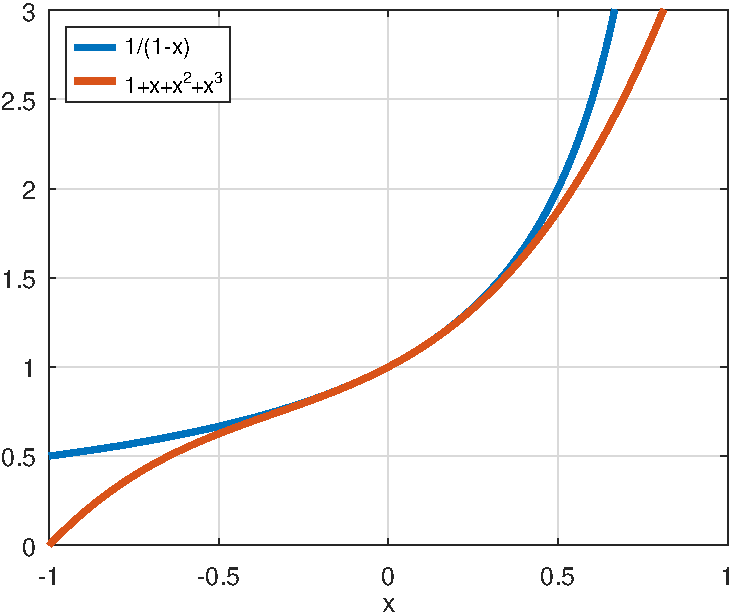
\includegraphics[width=0.4\textwidth]{figs/oneover.pdf} \quad 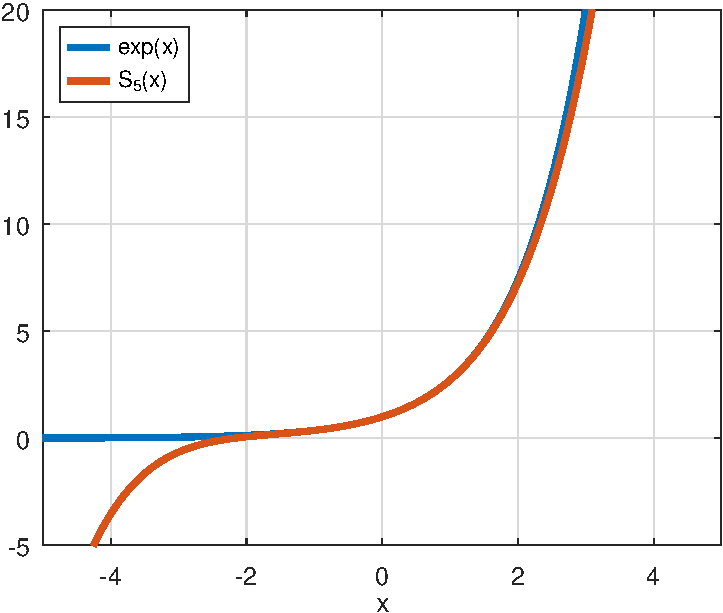
\includegraphics[width=0.4\textwidth]{figs/expsfive.pdf}}

We can multiply series, but only with effort. For example, here is the product of the two series:
\begin{align*}
g(x) &= \frac{e^x}{1-x} = \frac{1}{1-x} \, e^x = \left(1 + x + x^2 + x^3 + \dots\right) \,\left(1 + x + \frac{x^2}{2} + \frac{x^3}{3!} + \dots\right) \\
  &= 1 + 2x + \frac{5}{2} x^2 + \dots
\end{align*}
Computing the coefficients of the first few terms is like multiplying long polynomials, which is tedious.  However, the result is reasonable, and it looks like the figure below.

\bigskip
\centerline{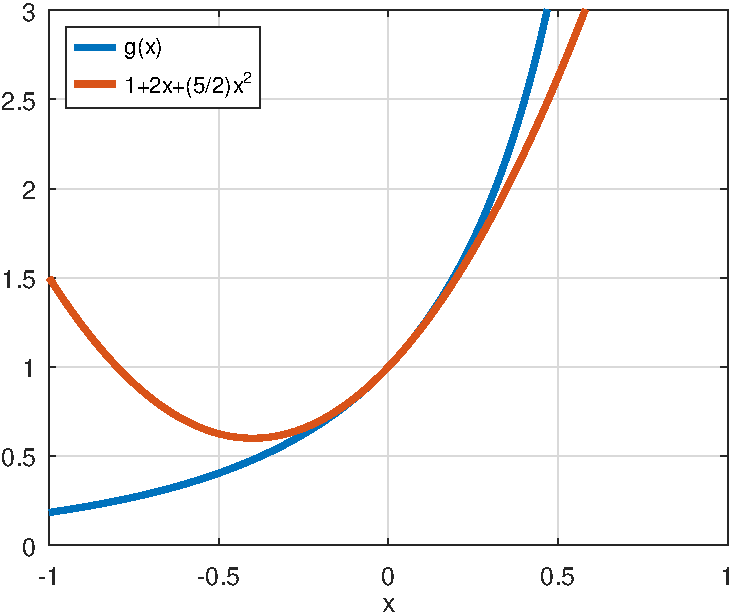
\includegraphics[width=0.4\textwidth]{figs/matching.pdf}}

Here is the Matlab code to make the last figure:
\begin{mVerb}
>> x = -1:.01:1;
>> plot(x,exp(x)./(1-x),x,1+2*x+(5/2)*x.^2)
>> axis([-1 1 0 3]),  grid on,  xlabel x
>> legend('g(x)','1+2x+(5/2)x^2','location','northwest')
\end{mVerb}
\end{document}
